\documentclass[11pt]{article}

\usepackage[letterpaper,margin=1in]{geometry}
\usepackage[T1]{fontenc}
\usepackage[utf8]{inputenc}
\usepackage{lmodern}
\usepackage{microtype}
\usepackage{enumitem}
\usepackage{xcolor}
\usepackage{hyperref}
\usepackage[strings]{underscore} % allow _ in text

\usepackage[numbers]{natbib} %removed cite package
\usepackage{csquotes}
\usepackage{adjustbox}
\usepackage{listings}
\usepackage{caption}   

\usepackage{graphicx}   % for \includegraphics
\usepackage{caption}    % better caption control inside minipage
\usepackage{subcaption} % optional, but useful if you want subfigures later


\hypersetup{
  colorlinks=true,
  linkcolor=blue!60!black,
  urlcolor=blue!60!black,
  citecolor=blue!60!black
}
\setcounter{secnumdepth}{1}
% Compact lists
\setlist[itemize]{leftmargin=1.2em,itemsep=0.3em,topsep=0.3em}
\setlist[enumerate]{leftmargin=1.4em,itemsep=0.3em,topsep=0.3em}

% Handy macros used in your text
\newcommand{\BPNoise}{\textsc{BP-Noise}}
\newcommand{\AmpMod}{\textsc{AmpMod}}
\newcommand{\LossSelect}{\textbf{Loss Selection}}
\newcommand{\SynthSelect}{\textbf{Synthesis Selection}}
\newcommand{\PeriodicLoss}{\textbf{Loss Landscape Navigation}}
\newcommand{\OutDomain}{\textbf{Out-Domain Generation}}
\newcommand{\DTWEnv}{\textsc{DTW\_Envelope}}
\newcommand{\SIMSESpec}{\textsc{SIMSE\_Spec}}
\newcommand{\LoneSpec}{\textsc{L1\_Spec}}
\newcommand{\JTFS}{\textsc{JTFS}}

\title{\vspace{-0.5em}Author Response for T-ASL-11868-2025\\
\large Manuscript: \emph{Evaluating Sound Similarity Metrics for Differentiable, Iterative Sound-Matching}}
\author{}
\date{}

\begin{document}
\maketitle
\vspace{-1.25em}

\noindent Dear Editor Alberto Bernardini, \\
\noindent
We'd like to thank you and the reviewers for the thoughtful and constructive feedback on our manuscript. We have carefully considered all comments and revised the manuscript accordingly. Here you will find our detailed point-by-point response to the feedback. 

For each reviewer, we first provide the review in full, with the key concerns numbered and in bold. Below the full review, we address the concerns in dedicated sections. Each section contains the reviewer's key requests or issues, followed by our response. Some revisions address more general concerns expressed in the body of the reviews (\nameref{R1.1} and \nameref{R1.2} for example). As such, for the sake of brevity we took the liberty to paraphrase the reviewer's requests and concerns as accurately as possible when necessary. 

\medskip
\noindent
We hope the revisions address all concerns and improve the clarity and quality of the manuscript.

\noindent Sincerely, Amir Salimi, Abram Hindle, Osmar R. Za{\"i}ane

\section{Reviewer 1}
\subsection{Original Review}
\noindent
The Introduction section lacks a clear articulation of the central research question early on. The core problem that no single loss function performs optimally across synthesizer types is buried within extended historical context and repeated definitions. Moreover, the use of a single subsection label (A. Digital Synthesis with Sound-Matching) without any follow-up sections is structurally inconsistent. \textbf{(R1.1) We recommend tightening the Introduction to focus more directly on problem motivation and contribution, and removing or completing the subsection structure.} \\
\textbf{(R1.2) The current division of the manuscript into Introduction, Background, and Past Works results in significant conceptual overlap and repetition.} Historical framing, loss function taxonomy, and method classification are spread across all three sections. \textbf{A clearer organizational approach would be to merge Background, and Past Works into a unified Background and Related Work section, where formal definitions, theoretical framing, and literature review are presented coherently.} This would allow the Introduction to focus solely on the motivation, problem framing, and contribution. \\
Section IV titled ``Programs, Methodology, and Results'' is overloaded and blends experimental setup with results and interpretation. \textbf{(R1.3) For clear clarity and alignment with structural norms, we recommend splitting this into three sections: (1) Experimental Setup (including synthesizer programs, loss definitions, optimization procedure); (2) Experimental Results (performance metrics, statistical tests, and rankings); and (3) Discussion (qualitative interpretation, synthesis-specific observations, and practical implications).} \\
Conceptually, the work serves primarily as a benchmarking study rather than a novel methodological contribution. While the comparison is comprehensive, the novel losses (DTW\_Envelope, SIMSE\_Spec) are adaptations of known techniques and are not framed with sufficient theoretical justification. \textbf{(R1.4) There is also limited interpretability analysis; for example, the paper does not explore why DTW performs well on modulated noise or why SIMSE outperforms L1 in certain scenarios.} Additionally, the synthesizers used are very simple (only 2--3 parameters), and all experiments are conducted in-domain, limiting the generalizability of the findings to real-world synthesis environments with more complex parameter spaces or out-of-domain targets. \\
\textbf{(R1.5) The manuscript would also benefit from clearer practical implications.} While the authors argue that sound-matching is a creative process and reject the idea of a universal loss, they stop short of offering actionable heuristics. \textbf{Some guidance (e.g., Use DTW for AM synthesis; SIMSE for subtractive synthesis) would strengthen the paper’s relevance to practitioners.} \\
\textbf{(R1.1) The paper would be improved by formally stating additional hypotheses that are currently only implicit.} For example, the observed agreement between manual and automatic evaluation metrics, the effectiveness of the novel losses, and the usability of iterative optimization as a general strategy are all important insights, but are not positioned as testable hypotheses upfront. \\
\textbf{Suggested Actions for Revision:}
\begin{enumerate}
  \item \textbf{(R1.1) Clearly state additional hypotheses regarding metric agreement, perceptual evaluation, and loss novelty.}
  \item \textbf{(R1.4) Deepen the technical and perceptual justification for DTW\_Envelope and SIMSE\_Spec.}
  \item \textbf{(R1.5) Add qualitative or spectral analyses of where specific losses succeed or fail.}
  \item \textbf{(R1.6) Expand discussion to address applicability to more complex or real-world synthesizers.}
  \item \textbf{(R1.7) Provide practical takeaways or usage guidelines for different loss-synth combinations.}
  \item \textbf{(R1.3) Restructure the manuscript to clarify the boundary between methodology, results, and discussion.}
\end{enumerate}

\subsection*{R1.1: Introduction Clarity}
\label{R1.1}
\noindent\textbf{Reviewer:}\\
\textbf{We recommend tightening the Introduction to focus more directly on problem motivation and contribution, and removing or completing the subsection structure.
\\}

\noindent\textbf{Response:} \\
We agree with the reviewer’s comment regarding lack of clarity and focus in the Introduction. The Introduction has been revised accordingly: 
\begin{itemize}
  \item The Introduction is now a single continuous section, without subsection headings.  
  \item We have removed unnecessary historical context and repeated definitions, reducing the length by roughly 25\%. We moved some of this material to the new \emph{Background and Related Work} section.  
  \item The central hypothesis now appears at the beginning of the third paragraph (previously it appeared mid-way through paragraph 10).  
  \item In addition to the main hypothesis, we have added three explicit research questions, covering metric agreement (Q1), the utility of novel DTW and SIMSE losses (Q2), and the viability of iterative optimization (Q3).  These are stated directly after the central hypothesis:

  \begin{displayquote}
     Beyond this central hypothesis, we also investigate three additional research questions: (Q1) To what extent do automatic evaluation metrics agree with manual listening tests? (Q2) Can loss functions based on Dynamic Time Warping (DTW) and Scale-Invariant Mean Squared Error (SIMSE) provide advantages over SOTA loss functions, and under what conditions?
    (Q3) Is iterative differentiable optimization a viable strategy for design of sound-matching experiments?
\end{displayquote}

  \item The Introduction concludes with a concise statement of our contributions:

  \begin{displayquote}
      The contributions of this paper include (1) an evaluation of multiple differentiable losses across multiple synthesis methods, (2) the introduction and justification of loss functions utilizing DTW and SIMSE (3) a discussion on the utility and agreement between manual and automatic evaluation metrics (4) a nomenclature of different sound-matching approaches and unsolved issues in the field. 
  \end{displayquote}
\end{itemize}

\subsection{R1.2 Improve Background and Related Work}
\label{R1.2}
\noindent\textbf{Reviewer:}\\
\noindent\textbf{The current division of the manuscript into Introduction, Background, and Past Works results in significant conceptual overlap and repetition. Historical framing, loss function taxonomy, and method classification are spread across all three sections. A clearer organizational approach would be to merge Background, and Past Works into a unified Background and Related Work section, where formal definitions, theoretical framing, and literature review are presented coherently. This would allow the Introduction to focus solely on the motivation, problem framing, and contribution.}\\

\noindent\textbf{Response:} \\
We agree that the organization and writing in these sections could be improved. We merged \emph{Background} and \emph{Past Works} into a unified \emph{Background and Related Work} section. Major applied major edits and rewrites to these sections to improve reading and remove redundancies between the various subsections while taking precautions in compromising the flow.
The \emph{background and Related Work} section contains the following topics in order:  
\begin{itemize}
  \item A formal definition of sound-matching and its components
  \item Definitions of synthesizers, losses, and optimization heuristics,  
  \item A chronological review of prior sound-matching approaches
  \item A discussion of gaps in the field and four critical issues.
  \item A justification for our methodology, and how our experiments address two of the critical issues (Loss and Synthesizer selection).
\end{itemize}


\subsection*{R1.3 Clarify the boundary between methodology, results, and discussion.}
\label{R1.3}
\noindent\textbf{Reviewer:}\\
\textbf{Section IV titled ``Programs, Methodology, and Results'' is overloaded and blends experimental setup with results and interpretation. For clear clarity and alignment with structural norms, we recommend splitting this into three sections: (1) Experimental Setup (including synthesizer programs, loss definitions, optimization procedure); (2) Experimental Results (performance metrics, statistical tests, and rankings); and (3) Discussion (qualitative interpretation, synthesis-specific observations, and practical implications).}
\\

\noindent\textbf{Response:} \\
We agree that the earlier draft blurred the boundaries between setup, results, and discussion. In the revised manuscript we implemented the reviewer’s suggestion as follows:

\begin{itemize}
  \item \textbf{III. Experimental Setup} (Sections III-A–E) now exclusively describes the methodological components: the synthesizer programs, the definitions of losses, the optimization procedure, evaluation metrics, and statistical tests. Each subsection is focused on describing how the experiments are designed, without interpretation of outcomes. For instance, the synthesizer section defines parameter ranges, while the evaluation section specifies how statistical significance is tested.  (he only partial overlap is at the beginning of the \textbf{III-F Best Performers for Each Program}, which transitions between results and discussion.

  \item Experimental findings are presented in \textbf{III-F Best Performers for Each Program} and \textbf{III-G Consistency in Rankings}, which together form the \emph{Results} component. Section III-F reports which losses performed best for each synthesizer, while Section III-G quantifies the consistency of rankings across bootstrap resamples. Keeping all numerical findings here avoids overlap with later interpretation.  

  \item \textbf{IV. Discussion} then provides the qualitative interpretation, structured into four dedicated subsections:  
    \begin{enumerate}
      \item \textbf{IV-A. Key Findings}: summarizes the central empirical trends, such as the dependency of loss performance on synthesis method.  
      \item \textbf{IV-B. Practical Recommendations} : translates results into concrete recommendations for practitioners and researchers.  
      \item \textbf{IV-C. Illustrating Loss Landscapes} : adds visualizations that explain why certain losses succeed or fail in specific contexts.  
      \item \textbf{IV-D. Applicability to More Complex Synthesizers} : discussion on how observed patterns extend beyond the simplified testbed to richer, real-world synthesizers.  
    \end{enumerate}

  \item To improve clarity, we also relocated explanatory material about experiment design (e.g., parameter settings, optimizer configuration) previously scattered across the results section into Sections III-A–E, so that the results sections are strictly empirical while the discussion is interpretive.  
\end{itemize}

Overall, this restructuring produces a clearer separation of topics: methodology is isolated in Section III-A–E, empirical findings are concentrated in Section III-F–G, and broader interpretation is reserved for Section IV. We believe this major restructuring and rewrites of appropriate sections has improved flow of the manuscript and made the boundary between methodology, results, and discussion much clearer.

\subsection*{R1.4 Justification for \DTWEnv{} and \SIMSESpec}
\label{R1.4}
\noindent\textbf{Reviewer:} \\
\noindent While the comparison is comprehensive, the novel losses (DTW\_Envelope, SIMSE\_Spec) are adaptations of known techniques and are not framed with sufficient theoretical justification. 

\noindent\textbf{Response:} \\
We have expanded the theoretical justifications for DTW\_Envelope and \SIMSESpec{} in subsection \textbf{II.C Sound Representation and Loss Functions}. In \textbf{II.C.2 Fourier Spectrograms}, we theorize the possible application of SIMSE as an alternative to L1:
\begin{displayquote}
    A common limitation of spectrogram-based losses is their sensitivity to global gain: two signals with identical spectral shape but different overall amplitude can yield large errors under L1/L2 norms. 
    Here we propose and test Scale-Invariant Mean Squared Error (SIMSE) as an alternative to L1/L2 norms in spectrogram comparisons. SIMSE normalizes the amplitudes before comparison and emphasizes proportional differences in spectral envelopes~\cite{barron2014shapessimse}. 
    Perceptually, listeners are often tolerant of loudness changes while remaining sensitive to timbral shape, therefore this property could be advantageous for subtractive synthesis, where filter cutoffs reshape spectral balance without predictable changes in total energy. Although SIMSE has been applied in other contexts such as audio reconstruction, to our knowledge its use as a differentiable spectrogram loss in iterative sound-matching is novel.
\end{displayquote}

 In \textbf{II.C.4 Dynamic Time Warping} For DTW\_Envelope, we clarify its perceptual motivation: aligning amplitude envelopes is crucial for AM synthesis, where traditional spectrogram L1 distances fail to capture similarity: 
 \begin{displayquote}
     DTW provides robustness to local temporal shifts, making it well suited for comparing modulated signals where the perceptual similarity lies in envelope dynamics rather than precise onset alignment. 
    For example, two tremolo signals with slightly different phase are perceptually similar but would appear distant under spectrogram L1. 
    A possible use case to consider is the application of DTW to amplitude envelopes, which may be able to match two sounds with identical rates of loudness modulation regardless of alignments. 
    To our knowledge, DTW applied in this way has not been used as a loss in sound-matching (whether differentiable and iterative or not).
 \end{displayquote}
 
 We explicitly frame these losses not as wholly new techniques, but as carefully adapted methods tested in an iterative differentiable setting, a contribution that has not previously been made.  

We did not modify the definitions in \textbf{III.A Loss Function Implementation Details}, dedicating this section to only technical explanations. 

\subsection*{R1.5 Analyses of where specific losses succeed or fail.}
\label{R1.5}
\noindent\textbf{Reviewer:} \\
\textbf{Add qualitative or spectral analyses of where specific losses succeed or fail}\\

\noindent\textbf{Response:} \\
This is an interesting suggestion. Our original experiments were designed to emphasize quantitative, statistically robust measurements of loss function performance, which is why we initially avoided focusing on individual examples of sounds, spectrograms, or loss landscapes (to reduce the risk of cherry-picking). However, illustrative examples can provide helpful intuition for readers and motivate future research. However, we believe that an analysis of loss landscapes (rather than spectrograms or qualitative tests) is a more useful approach to a discussion on where and \textit{why} losses might succeed or fail.

To this end, we have added a new Section \textbf{IV.C llustrating Loss Landscapes} where qualitative visualizations of loss landscapes  are added. These examples highlight why specific losses may succeed or fail and reinforce the broader importance of loss landscapes in assessing the appropriateness of similarity measures~\cite{vahidi2023mesostructures,turian2020sorry}, supporting our argument that effective navigation of loss landscapes represents an important gap in current knowledge and a promising direction for future work:


\begin{displayquote}
    Figure~\ref{fig:loss_landscape_noisebp} shows the HP-Noise results. \LoneSpec{}, \SIMSESpec{}, and \JTFS{} exhibit clear minima at the correct parameter (red dashed line), whereas \DTWEnv{} remains relatively flat, making gradient-based optimization more difficult.

    Figure~\ref{fig:loss_landscape_ampmod} shows the S-Noise-AM results. Here, \DTWEnv{} produces the smoothest and most informative landscape, while spectrogram losses are minimized near the target but lack consistent correlation with parameter distance. \JTFS{} remains largely flat. This aligns with \DTWEnv's superior performance in amplitude-modulated synthesis observed in our experiments.
\end{displayquote}

\begin{figure*}[ht]
    \centering
    \begin{minipage}[t]{0.48\textwidth}
        \centering
        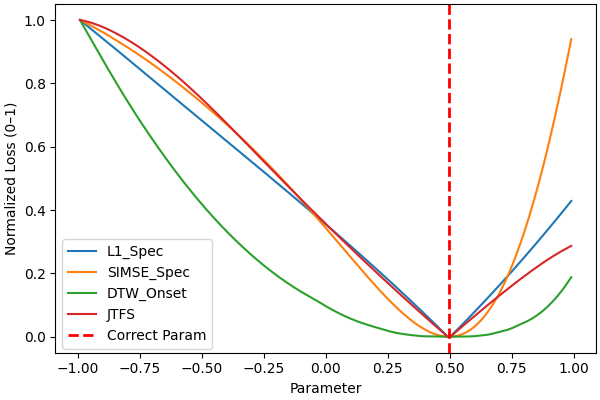
\includegraphics[width=\linewidth]{images/experiment_plots/comparing_loss_landscapes_normalized.png}
        \caption{Loss landscapes for \BPNoise{} with only a high-pass filter parameter. 
        \LoneSpec{}, \SIMSESpec{}, and \JTFS{} show clear global minima near the correct parameter, while \DTWEnv{} remains flat around the target.}
        \label{fig:loss_landscape_noisebp}
    \end{minipage}%
    \hfill
    \begin{minipage}[t]{0.48\textwidth}
        \centering
        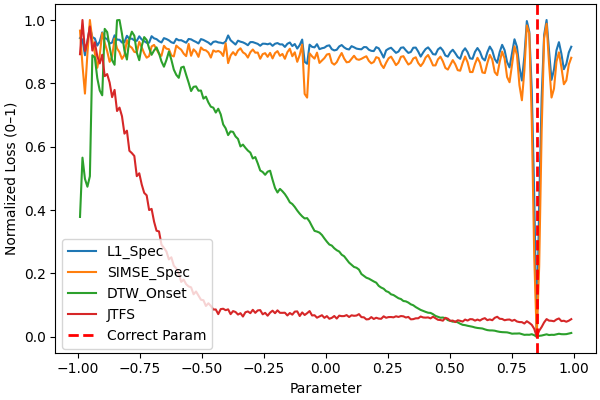
\includegraphics[width=\linewidth]{images/experiment_plots/comparing_lanscapes_1_1d_normalized.png}
        \caption{Loss landscapes for a simplified \AmpMod{} synthesizer with only amplitude modulation parameter. 
        \DTWEnv{} exhibits the smoothest and most informative landscape, explaining its superior performance in amplitude-modulated synthesis.}
        \label{fig:loss_landscape_ampmod}
    \end{minipage}
\end{figure*}

While this may not be the "qualitative" or "spectral" analysis, we believe it is instructive on the mechanisms underlying our quantitative findings and highlight the importance of loss landscape navigation as an open area for future research.

\subsection*{R1.6 Applicability to more complex or real-world synthesizers.}
\label{R1.6}
\noindent\textbf{Review:} \\
\noindent \textbf{Expand the discussion to address applicability to more complex or real-world synthesizers}
\\

\noindent\textbf{Response:} \\
We added a new subsection, \textbf{IV.D Applicability to More Complex Synthesizers}, that explicitly discusses how the insights from our controlled two-parameter DSP-based synthesizers generalize to richer synthesizers with many parameters and complex routing. While acknowledging the limitations of our simplified test bed, we argue that the observed dependencies between synthesis method and loss function remain informative even in more complex settings:

\begin{displayquote}
    The experiments in this study were conducted with differentiable synthesizers chosen to isolate fundamental synthesis principle with 2 parameters each. While this level of simplicity facilitates controlled comparisons, it does not fully capture the richness of real-world synthesizers, which can have hundreds of parameters with various routes. As a result, the extent of the generalizability of our findings does require further research. 

    Nonetheless, we believe that the insights here can extend naturally to more complex domains. Depending on the feature of interest, the observed dependence of loss performance on synthesis method is will likely remain stable even with added complexities such as layers of modulation, filtering, or nonlinearity. 
    
    \DTWEnv{} measures very specific features of audio, and its use in the recommended settings---where low frequency amplitude modulation matching is required---would likely yield the desired results regardless of synthesizer complexity. Likewise, the use of \SIMSESpec{} or \LoneSpec{} for matching filter cut-offs is likely to be successful regardless of the underlying sound. 
    \end{displayquote}
    

\subsection{R1.7 Provide practical takeaways}
\label{R1.7}
\noindent\textbf{Review:} \\
\noindent \textbf{Provide practical takeaways or usage guidelines for different loss-synth combinations. } 
\\

\noindent\textbf{Response} \\
We introduced a new subsection, \textbf{IV.B Practical Recommendations}, which distills our findings into actionable heuristics for practitioners. 

\begin{displayquote}
    Based on our findings, several actionable guidelines emerge. These heuristics can guide practitioners in selecting appropriate similarity measures and synthesis methods for future sound-matching experiments.
\begin{itemize}
    \item In lieu of listening tests, MSS or P-Loss are generally useful for large-scale benchmarking, but confirm conclusions with manual listening when accuracy in isolated cases is important. 
    \item For amplitude-modulated synthesis, DTW-based losses (e.g., \DTWEnv{}) are recommended over spectrogram based and JTFS. 
    \item For subtractive/noise-filtered synthesis, spectrogram based losses are most effective. Based on our results, SIMSE appears to be the better method of spectrogram comparisons relative to L1, but the amplitude agnosticism of SIMSE likely plays a role in its poor performance in additive synthesis.  
    \item In our amplitude modulation experiments, \JTFS{} did not outperform other measures, contradicting prior claims of its superiority for mesostructures~\cite{vahidi2023mesostructures}. Thus, our results call into question its effectiveness as a general mesostructure measure
    \item Iterative differentiable optimization via Faust-to-JAX is a viable strategy for defining various differentiable DSP functions, requiring only modest hardware resource and providing a more natural approach to synthesizer definition.
\end{itemize}

\end{displayquote}
\section{Reviewer 2}
\subsection{Original Review}
\noindent
The paper considers the evaluation of different audio similarity metrics for sound matching applications.  The authors categorize prior methods largely as direct optimization via gradient-free iterative search or open-loop inference via a supervised deep learning model.  Moreover, different approaches which may or may not accommodate out-of-domain sounds.  Accordingly, the authors propose the combined use of differentiable synthesizers and closed-loop iteration as a sound means of achieving synthesizer sound matching, effectively combining the advantages of otherwise disparate methods (i.e. access to gradients while iteratively improving matching results).  Additionally, within their evaluation of different similarity metrics (parameter losses, spectral distances, etc.), they also introduce a DTW-based similarity metric to partially neutralize the effect of time alignment on similarity scores.  A primary conclusion of the work is that there is no one best sound similarity measure capable of working across all synthesizers.  \\
The subject matter of the work is relevant, the experimental setup is satisfactory, and I do not have reason to doubt the correctness of their analysis.  However, my primary concerns with this work are that:  
\begin{enumerate}
  \item \textbf{(R2.1) It is not clear what the proposed method really is, and the paper reads largely as a readout of evaluations that were conducted by the authors.}  
  \item \textbf{(R2.2) The authors claim that differentiable iterative sound matching is largely unexplored, encouraging development of techniques in this area.}  
    \begin{itemize}
      \item \textbf{Barkan et. al, ``Inversynth II: Sound Matching via Self-Supervised Synthesizer-Proxy and Inference-Time Finetuning'' explored precisely this, training an initial ``one-shot'' supervised model, and then performing inference-time optimization, updating model weights to improve the matching against test audio.  Moreover, their use of a synthesizer-proxy negates the explicit need of implementing the synthesizer math differentiably, while still falling under the category of differentiable iterative sound matching.}  
      \item \textbf{Cherep et. al, ``Creative Text-to-Audio Generation via Synthesizer Programming'' uses a differentiable synthesizer and the CLAP score as a similarity metric for iterative optimization.  While the authors lean into synthesizer sound matching against a text query, the method would be readily applicable to audio-to-audio sound matching using the CLAP audio tower alone.}  
    \end{itemize}
  \item \textbf{(R2.3) This work addresses the problems on ``Loss Selection'' and ``Synthesis Selection.''  However, the results as presented here are largely inconclusive (i.e. it is not imminently clear how to select losses/synthesizer pairings), leaving very little in the way of clear takeaways sparking future research.}
\end{enumerate}

\subsection{R2.1 Clarity of proposed method}
\label{R2.1}
\noindent\textbf{Review:}
\noindent \textbf{It is not clear what the proposed method really is, and the paper reads largely as a readout of evaluations. } 
\\

\noindent\textbf{Response:} \\
We have taken several measures to clarify the methodology and ensure that the paper is not read ``merely as a set of experiments''.  

\medskip
\noindent In \textbf{II.B Digital Signal Processing and Synthesis}, we state the importance of isolated experiments:
\begin{displayquote}
    
Other synthesis methods studied in \textit{isolation} include additive and subtractive synthesis~\cite{engel2020ddsp,masuda2023improving,salimi2020make} and physical modeling~\cite{riionheimo2003parameter,han2024learning}. By \textit{isolation}, we mean settings where the effect of individual parameters on the output sound remains tractable. For example, we exclude studies using commercial Virtual Studio Technology (VST) which can obscure the interactions between modules, losses, and outputs. 
\end{displayquote}

\noindent To further clarify the methodology and its importance, we have added a new subsection, \textbf{II.H What Approach Should We Take?} placed immediately before the Methodology section. This subsection clarifies our experimental design and explains why our contribution is unique. Specifically, we use:  
\begin{enumerate}
  \item Simple differentiable DSP synthesizers to isolate synthesis--loss interactions,  
  \item Multiple losses tested side by side within the same framework, and  
  \item Direct gradient descent optimization without neural proxies.  
\end{enumerate}

This quote from the aforementioned section in the paper makes clear that our work is not simply a report of evaluations, but a controlled benchmarking study designed to reveal how losses and synthesis methods interact: 

\begin{displayquote}
    We argue that isolated benchmarking is a necessary precursor to building robust, generalizable sound-matching systems. To address the problems of \LossSelect{} and \SynthSelect{}, we adopt a methodology with three key characteristics that have not previously appeared together.

\begin{enumerate}
    \item Use simple differentiable synthesizers built from common DSP functions (oscillators, filters, envelopes) to address the \SynthSelect{} problem. Restricting to small-scale, low-parameter models avoids the confounding effects of neural proxies or embedding models, enabling direct analysis of how synthesis method interacts with loss functions. 
    \item Evaluate experiments under multiple loss functions to address the \LossSelect{} problem. Prior work has typically tested losses in isolation, making direct comparisons rare\cite{vahidi2023mesostructures}.  
    \item Optimize synthesizer parameters directly with gradient descent, without neural approximations. This complements prior proxy-based methods by providing the missing “low-level experiments” that clarify fundamental interactions between DSP functions and similarity measures. 
\end{enumerate}

Together, these design choices supply the controlled experimental evidence missing from the literature, 
clarifying how losses and synthesis methods interact in differentiable, iterative settings, 
and offering insights likely to generalize to more complex domains.

\end{displayquote}


\medskip
\noindent We restate our methodology in the opening paragraph of the \textbf{III. Experimental Setup} section:

\begin{displayquote}
    At a glance, our methodology is to conduct controlled, low-level differentiable experiments—without proxy networks—by pairing four DSP-based synthesizers with four differentiable loss functions. We optimize parameters directly via gradients in order to isolate loss–synthesizer interactions. This controlled setup systematically evaluates the performance of iterative sound-matching pipelines, where “performance” is defined as the similarity of the synthesized output to a target. Similarity is assessed with P-Loss, MSS, and—most importantly—manual listening tests. This design allows us to directly test our central hypothesis: that the effectiveness of a loss function depends on the synthesis method, and that no universal “best” similarity measure exists.
\end{displayquote}

\subsection*{R2.2 Relation to prior work}
\noindent \textbf{The authors claim that differentiable iterative sound matching is largely unexplored, but prior work (Barkan et al., Cherep et al.) could be considered in this category.}\\

\noindent\textbf{Response:} \\
We thank the reviewer for pointing out sound-matching works which fall under the ``differentiable and iterative'' description that were not covered in our literature review. We believe that the term ``under-explored'' is perhaps more appropriate. We've added these works to \textbf{Table 1} which provides a summary of important previous works, and discussed these works in more detail in the \textbf{II.F Historical Framing of Sound-Matching} section: 
\begin{itemize}
  \item \textbf{Barkan et al. (Inversynth II):} Their work relies on neural proxies for the synthesizer, with inference-time finetuning of the encoder. This constitutes iterative optimization, but the optimization occurs on an approximate model rather than directly on differentiable DSP functions. By contrast, our approach avoids proxy error and directly analyzes how losses behave relative to known synthesis structures.  
  \item \textbf{Cherep et al.:} Their work uses CLAP embeddings with evolutionary search for text-to-audio tasks. While applicable to audio-to-audio matching, CLAP acts as a black-box representation and does not isolate loss--synth interactions. Our approach is complementary, focusing on controlled experiments with simple differentiable DSP synthesizers to expose the strengths and weaknesses of different similarity measures.  In addition, embedding models such as CLAP use simpler representations at their core, commonly the Fourier transformations, and our work explores the low level functions that are often used for the training of embedding models.
\end{itemize}
Looking at these works, we see that our contribution is distinct: we provide the missing \textbf{low-level benchmarking} of loss functions across multiple synthesis methods, which is not addressed by proxy-based or embedding-based approaches.

\subsection*{R2.3 Clear takeaways}
\noindent\textbf{Review:}
\textbf{This work addresses the problems on ``Loss Selection'' and ``Synthesis Selection.''  However, the results as presented here are largely inconclusive (i.e. it is not imminently clear how to select losses/synthesizer pairings), leaving very little in the way of clear takeaways sparking future research.\\}

\noindent\textbf{Response:} \\
In the revised paper, we've added two sections which address the valid issues raised here and by Reviewer 1. 

\begin{itemize}
  \item We added a new subsection, \emph{Applicability to More Complex Synthesizers}, that explicitly discusses how the insights from our controlled two-parameter DSP-based synthesizers generalize to richer synthesizers with many parameters and complex routing. While acknowledging the limitations of our simplified testbed, we argue that the observed dependencies between synthesis method and loss function remain informative even in more complex settings.
  \item We introduced a new subsection, \emph{Practical Recommendations}, which distills our findings into actionable heuristics for practitioners. DTWEnv is recommended for amplitude-modulated synthesis, SIMSE for subtractive/noise-filtered synthesis, and MSS or P-Loss as large-scale proxies for sound-matching evaluation (with manual validation being strongly advised). We also note that our results challenge prior claims about JTFS’s universal superiority for mesostructures.

\end{itemize}

For a more detailed response, see our response to the Reviewer.1 in Sections~\nameref{R1.6} and \nameref{R1.7}.


\bibliographystyle{IEEEtran}
\bibliography{references}

\end{document}
